% Options for packages loaded elsewhere
\PassOptionsToPackage{unicode}{hyperref}
\PassOptionsToPackage{hyphens}{url}
\PassOptionsToPackage{dvipsnames,svgnames,x11names}{xcolor}
%
\documentclass[
  letterpaper,
  DIV=11,
  numbers=noendperiod]{scrartcl}

\usepackage{amsmath,amssymb}
\usepackage{iftex}
\ifPDFTeX
  \usepackage[T1]{fontenc}
  \usepackage[utf8]{inputenc}
  \usepackage{textcomp} % provide euro and other symbols
\else % if luatex or xetex
  \usepackage{unicode-math}
  \defaultfontfeatures{Scale=MatchLowercase}
  \defaultfontfeatures[\rmfamily]{Ligatures=TeX,Scale=1}
\fi
\usepackage{lmodern}
\ifPDFTeX\else  
    % xetex/luatex font selection
\fi
% Use upquote if available, for straight quotes in verbatim environments
\IfFileExists{upquote.sty}{\usepackage{upquote}}{}
\IfFileExists{microtype.sty}{% use microtype if available
  \usepackage[]{microtype}
  \UseMicrotypeSet[protrusion]{basicmath} % disable protrusion for tt fonts
}{}
\makeatletter
\@ifundefined{KOMAClassName}{% if non-KOMA class
  \IfFileExists{parskip.sty}{%
    \usepackage{parskip}
  }{% else
    \setlength{\parindent}{0pt}
    \setlength{\parskip}{6pt plus 2pt minus 1pt}}
}{% if KOMA class
  \KOMAoptions{parskip=half}}
\makeatother
\usepackage{xcolor}
\setlength{\emergencystretch}{3em} % prevent overfull lines
\setcounter{secnumdepth}{5}
% Make \paragraph and \subparagraph free-standing
\makeatletter
\ifx\paragraph\undefined\else
  \let\oldparagraph\paragraph
  \renewcommand{\paragraph}{
    \@ifstar
      \xxxParagraphStar
      \xxxParagraphNoStar
  }
  \newcommand{\xxxParagraphStar}[1]{\oldparagraph*{#1}\mbox{}}
  \newcommand{\xxxParagraphNoStar}[1]{\oldparagraph{#1}\mbox{}}
\fi
\ifx\subparagraph\undefined\else
  \let\oldsubparagraph\subparagraph
  \renewcommand{\subparagraph}{
    \@ifstar
      \xxxSubParagraphStar
      \xxxSubParagraphNoStar
  }
  \newcommand{\xxxSubParagraphStar}[1]{\oldsubparagraph*{#1}\mbox{}}
  \newcommand{\xxxSubParagraphNoStar}[1]{\oldsubparagraph{#1}\mbox{}}
\fi
\makeatother


\providecommand{\tightlist}{%
  \setlength{\itemsep}{0pt}\setlength{\parskip}{0pt}}\usepackage{longtable,booktabs,array}
\usepackage{calc} % for calculating minipage widths
% Correct order of tables after \paragraph or \subparagraph
\usepackage{etoolbox}
\makeatletter
\patchcmd\longtable{\par}{\if@noskipsec\mbox{}\fi\par}{}{}
\makeatother
% Allow footnotes in longtable head/foot
\IfFileExists{footnotehyper.sty}{\usepackage{footnotehyper}}{\usepackage{footnote}}
\makesavenoteenv{longtable}
\usepackage{graphicx}
\makeatletter
\def\maxwidth{\ifdim\Gin@nat@width>\linewidth\linewidth\else\Gin@nat@width\fi}
\def\maxheight{\ifdim\Gin@nat@height>\textheight\textheight\else\Gin@nat@height\fi}
\makeatother
% Scale images if necessary, so that they will not overflow the page
% margins by default, and it is still possible to overwrite the defaults
% using explicit options in \includegraphics[width, height, ...]{}
\setkeys{Gin}{width=\maxwidth,height=\maxheight,keepaspectratio}
% Set default figure placement to htbp
\makeatletter
\def\fps@figure{htbp}
\makeatother

\KOMAoption{captions}{tableheading}
\usepackage{biblatex}
\usepackage{sectsty}
\sectionfont{\clearpage}
\ExecuteBibliographyOptions{sorting=none,defernumbers=true}
\makeatletter
\@ifpackageloaded{caption}{}{\usepackage{caption}}
\AtBeginDocument{%
\ifdefined\contentsname
  \renewcommand*\contentsname{Table of contents}
\else
  \newcommand\contentsname{Table of contents}
\fi
\ifdefined\listfigurename
  \renewcommand*\listfigurename{List of Figures}
\else
  \newcommand\listfigurename{List of Figures}
\fi
\ifdefined\listtablename
  \renewcommand*\listtablename{List of Tables}
\else
  \newcommand\listtablename{List of Tables}
\fi
\ifdefined\figurename
  \renewcommand*\figurename{Figure}
\else
  \newcommand\figurename{Figure}
\fi
\ifdefined\tablename
  \renewcommand*\tablename{Table}
\else
  \newcommand\tablename{Table}
\fi
}
\@ifpackageloaded{float}{}{\usepackage{float}}
\floatstyle{ruled}
\@ifundefined{c@chapter}{\newfloat{codelisting}{h}{lop}}{\newfloat{codelisting}{h}{lop}[chapter]}
\floatname{codelisting}{Listing}
\newcommand*\listoflistings{\listof{codelisting}{List of Listings}}
\makeatother
\makeatletter
\makeatother
\makeatletter
\@ifpackageloaded{caption}{}{\usepackage{caption}}
\@ifpackageloaded{subcaption}{}{\usepackage{subcaption}}
\makeatother

\ifLuaTeX
  \usepackage{selnolig}  % disable illegal ligatures
\fi
\usepackage[]{biblatex}
\addbibresource{references.bib}
\usepackage{bookmark}

\IfFileExists{xurl.sty}{\usepackage{xurl}}{} % add URL line breaks if available
\urlstyle{same} % disable monospaced font for URLs
\hypersetup{
  pdftitle={Tree object detection using airborne images and LiDAR point clouds},
  pdfauthor={Alexandre Bry},
  pdfkeywords={tree detection, deep learning},
  colorlinks=true,
  linkcolor={blue},
  filecolor={Maroon},
  citecolor={Blue},
  urlcolor={Blue},
  pdfcreator={LaTeX via pandoc}}


\title{Tree object detection using airborne images and LiDAR point
clouds}
\author{Alexandre Bry}
\date{2024-07-22}

\begin{document}
\maketitle
\begin{abstract}
This is the abstract. It can be on multiple lines and contain
\textbf{Markdown}.
\end{abstract}

\renewcommand*\contentsname{Table of contents}
{
\hypersetup{linkcolor=}
\setcounter{tocdepth}{3}
\tableofcontents
}

\section*{Introduction}\label{introduction}
\addcontentsline{toc}{section}{Introduction}

The goal of the internship was to study the possibility of combining
LiDAR point clouds and aerial images in a deep learning model to
identify individual trees. The two types of data are indeed
complementary, as point clouds capture geometric shapes, while images
capture colors. However, combining them into a format that allows a
model to handle them simultaneously is not a straightforward task
because they inherently have a very different spatial repartition and
encoding.

In this work, I focused on one specific deep learning model, and tried
to improve it by using more information from the LiDAR point cloud. To
do this, I had to create my own tree annotations dataset, with which I
also tried to study the ability of this new model to detect trees that
are covered by other trees.

\section{State-of-the-art}\label{state-of-the-art}

\subsection{Computer vision tasks related to
trees}\label{computer-vision-tasks-related-to-trees}

Before talking about models and datasets, let's define properly the task
that this project focused on, in the midst of all the various computer
vision tasks, and specifically those related to tree detection.

The first main differentiation between tree recognition tasks comes from
the acquisition of the data. There are some very different tasks and
methods using either ground data or aerial/satellite data. This is
especially true when focusing on urban trees, since a lot of street view
data is available \autocite{urban-trees}.

This leads to the second variation, which is related to the kind of
environment that we are interested in. There are mainly three types of
environments, which among other things, influence the organization of
the trees in space: urban areas, tree plantations and forests. This is
important, because the tasks and the difficulty depends on the type of
environment. Tree plantations are much easier to work with than
completely wild forests, while urban areas contain various levels of
difficulty ranging from alignment trees to private and disorganized
gardens and parks. For this project, we mainly focused on urban areas,
but everything should still be applicable to tree plantations and
forests.

Then, the four fundamental computer vision tasks have their application
when dealing with trees \autocite{olive-tree}:

\begin{itemize}
\tightlist
\item
  Classification, although this is quite rare for airborne tree
  applications since there are multiple trees on each image most of the
  time
\item
  Detection, which consists in detecting objects and placing boxes
  around them
\item
  Semantic segmentation, which consists in associating a label to every
  pixel of an image
\item
  Instance segmentation, which consists in adding a layer of complexity
  to semantic segmentation by also differentiating between the different
  instances of each class
\end{itemize}

These generic tasks can be extended by trying to get more information
about the trees. The most common information are the species and the
height, but some models also try to predict the health of the trees, or
their carbon stock.

In this work, the task that is tackled is the detection of trees, with a
special classification between several labels related to the
discrepancies between the different kinds of data. The kind of model
that is used would also have allowed to focus on some more advanced
tasks, by replacing detection with instance segmentation and asking the
model to also predict the species. But due to the difficulties regarding
the dataset, a simpler task with a simpler dataset was used, without
compromising the ability to experiment with different possible
improvements of the model. The difficulties and the experiments are
developed below.

\subsection{Datasets}\label{datasets}

\subsubsection{Requirements}\label{sec-sota-datasets-requirements}

Before presenting the different promising datasets and the reasons why
they were not fully usable for the project, let's enumerate the
different conditions and requirements for the tree instance segmentation
task:

\begin{itemize}
\tightlist
\item
  Multiple types of data:

  \begin{itemize}
  \tightlist
  \item
    Aerial RGB images
  \item
    LiDAR point clouds (preferably aerial)
  \item
    (Optional) Aerial infrared (CIR) images
  \end{itemize}
\item
  Tree crown annotations or bounding boxes
\item
  High-enough resolution:

  \begin{itemize}
  \tightlist
  \item
    For images, about 25~cm
  \item
    For point clouds, about 10~cm
  \end{itemize}
\end{itemize}

Here are the explanations for these requirements. As for the types of
data, RGB images and point clouds are required to experiment on the
ability of the model to combine the two very different kinds of
information they hold. Having infrared data as well could be beneficial,
but it was not necessary. Regarding tree annotations, it was necessary
to have a way to spatially identify them individually, using crown
contours or simply bounding boxes. Since the model outputs bounding
boxes, any kind of other format could easily be transformed to bounding
boxes. Finally, the resolution had to be high enough to identify
individual trees and be able to really use the data. For the point
clouds especially, the whole idea was to see if and how the topology of
the trees could be learnt, using at least the trunks and even the
biggest branches if possible. Therefore, even if they are not really
comparable, this is the reason why the required resolution is more
precise for the point clouds.

Unfortunately, none of the datasets that I found matched all these
criteria. Furthermore, I didn't find any overlapping datasets that I
could merge to create a dataset with all the required types of data. In
the next parts, I will go through the different kinds of datasets that
exist, the reasons why they did not really fit for the project and the
ideas I got when searching for a way to use them.

\subsubsection{Existing tree datasets}\label{existing-tree-datasets}

As explained above, there were quite a lot of requirements to fulfill to
have a complete dataset usable for the task. This means that almost all
the available datasets were missing something, as they were mainly
focusing on using one kind of data and trying to make the most out of
it, instead of trying to use all the types of data together.

The most comprehensive list of tree annotations datasets was published
in OpenForest \autocite{OpenForest}. FoMo-Bench \autocite{FoMo-Bench}
also lists several interesting datasets, even though most of them can
also be found in OpenForest. Without enumerating all of them, there were
multiple kinds of datasets that all have their own flaws regarding the
requirements I was looking for.

Firstly, there are the forest inventories. TALLO \autocite{TALLO} is
probably the most interesting one in this category, because it contains
a lot of spatial information about almost 500K trees, with their
locations, their crown radii and their heights. Therefore, everything
needed to localize trees is in the dataset. However, I didn't manage to
find RGB images or LiDAR point clouds of the areas where the trees are
located, making it impossible to use these annotations to train tree
detection.

Secondly, there are the RGB datasets. ReforesTree \autocite{ReforesTree}
and MillionTrees \autocite{MillionTrees} are two of them and the quality
of their images are high. The only drawback of these datasets is
obviously that they don't provide any kind of point cloud, which make
them unsuitable for the task.

Thirdly, there are the LiDAR datasets, such as \autocite{WildForest3D}
and \autocite{FOR-instance}. Similarly to RGB datasets, they lack one of
the data source for the task I worked on. But unlike them, they have the
advantage that the missing data could be much easier to acquire from
another source, since RGB aerial or satellite images are much more
common than LiDAR point clouds. However, this solution was abandoned for
two main reasons. First it is quite challenging to find the exact
locations where the point clouds were acquired. Then, even when the
location is known, it is often in the middle of a forest where the
quality of satellite imagery is very low.

Finally, I also found two datasets that had RGB and LiDAR components.
The first one is MDAS \autocite{MDAS}. This benchmark dataset
encompasses RGB images, hyperspectral images and Digital Surface Models
(DSM). There were however two major flaws. The obvious one was that this
dataset was created with land semantic segmentation tasks in mind, so
there was no tree annotations. The less obvious one was that a DSM is
not a point cloud, even though it is some kind of 3D information and was
often created using a LiDAR point cloud. As a consequence, I would have
been very limited in my ability to use the point cloud.

The only real dataset with RGB and LiDAR came from NEON
\autocite{NEONdata}. This dataset contains exactly all the data I was
looking for, with RGB images, hyperspectral images and LiDAR point
clouds. With 30975 tree annotations, it is also a quite large dataset,
spanning across multiple various forests. The reason why I decided not
to use it despite all this is that at the beginning of the project, I
thought that the quality of the images and the point clouds was too low.
Looking back on this decision, I think that I probably could have worked
with this dataset and gotten great results. This would have saved me the
time spent annotating the trees for my own dataset, which I will talk
more about later. My decision was also influenced by the quality of the
images and the point clouds available in the Netherlands, which I will
talk about in the next section.

\subsubsection{Public data}\label{public-data}

After rejecting all the available datasets I had found, the only
solution I had left was to create my own dataset. I won't dive too much
in this process that I will explain in Section~\ref{sec-dataset}. I just
want to mention all the publicly available datasets that I used or could
have used to create this custom dataset.

For practical reasons, the two countries where I mostly searched for
available data are France and the Netherlands. I was looking for three
different data types independently:

\begin{itemize}
\tightlist
\item
  RGB (and if possible CIR) images
\item
  LiDAR point clouds
\item
  Tree annotations
\end{itemize}

These three types of data are available in similar ways in both
countries, although the Netherlands have a small edge over France. RGB
images are really easy to find in France with the BD ORTHO
\autocite{IGN_BD_ORTHO} and in the Netherlands with the Luchtfotos
\autocite{Luchtfotos}, but the resolution is better in the Netherlands
(8~cm vs 20~cm). Hyperspectral images are also available in both
countries, although for those the resolution is only 25~cm in the
Netherlands.

As for LiDAR point clouds, the Netherlands have a small edge over
France, because they have already completed their forth version covering
the whole country with AHN4 \autocite{AHN4}, and are working on the
fifth version. In France, data acquisition for the first LiDAR point
cloud covering the whole country started a few years ago
\autocite{IGN_LiDAR_HD}. It is not yet finished, even though data is
already available for half of the country. The other advantage of the
data from Netherlands regarding LiDAR point clouds is that all flights
are performed during winter, which allows light beams to penetrate more
deeply in trees and reach trunks and branches. This is not the case in
France.

The part that is missing in both countries is related to tree
annotations. Many municipalities have datasets containing information
about all the public trees they handle. This is for example the case for
Amsterdam \autocite{amsterdam_trees} and Bordeaux
\autocite{bordeaux_trees}. However, these datasets cannot really be used
as ground truth for a custom dataset for several reasons. First, many of
them do not contain coordinates indicating the position of each tree in
the city. Then, even those that contain coordinates are most of the time
missing any kind of information allowing to deduce a bounding box for
the tree crowns. Finally, even if they did contain everything, they only
focus on public trees, and are missing every single tree located in a
private area. Since public and private areas are obviously imbricated in
all cities, it means that any area we try to train the model on would be
missing all the private trees, making the training process impossible
because we cannot have only a partial annotation of images.

The other tree annotation source that we could have used is Boomregister
\autocite{boomregister}. This work covers the whole of the Netherlands,
including public and private trees. However, the precision of the masks
is far from perfect, and many trees are missing or incorrectly
segmented, especially when they are less than 9~m heigh or have a crown
diameter smaller than 4~m. Therefore, even it is a very impressive piece
of work, we thought that it could not be used as training data for a
deep learning models due to its biases and imperfections.

\subsubsection{Dataset augmentation
techniques}\label{sec-sota-dataset-augment}

When a dataset is too small to train a model, there are several ways of
artificially enlarging it.

The most common way to do it is to randomly apply deterministic or
random transformations to the data, during the training process, to be
able to generate several unique and different realistic data instances
from one real data instance. There are a lot of different
transformations that can be applied to images, divided into two
categories: pixel-level and spatial-level \autocite{albumentations}.
Pixel-level transformations modify the value of individual pixels, by
applying different filters, such as random noise, color shifts and more
complex effects like fog and sun flare. Spatial-level transformations
modify the spatial arrangement of the image, without changing the pixel
values. In other words, these transformations move the pixels in the
image. The transformations range from simple rotations and croppings to
complex spatial distortions. In the end, all these transformations are
simply producing one artificial image out of one real image.

Another way to enlarge a dataset is to instead generate completely new
input data sharing the same properties as the initial dataset. This can
be done using Generative Adversarial Networks (GAN). These models
usually have two parts, a generator and a discriminator, which are
trained in parallel. The generator learns to produce realistic
artificial data, while the discriminator learns to identify real data
and artificial data produced by the generator. If the training is
successful, we can then use the generator and random seeds to generate
random but realistic artificial data similar to the dataset. This method
has for example been successfully used to generate artificial tree
height maps \autocite{gan_data_augment}.

\subsection{Algorithms and models}\label{algorithms-and-models}

In this section, the different algorithms and methods are grouped
according to the type of data they use as input.

\subsubsection{Images only}\label{images-only}

Then, there are methods that perform tree detection using only visible
or hyperspectral images or both. Several different algorithms have been
developed to analytically delineate tree crowns from RGB images, by
using the particular shape of the trees and its effect on images
\autocite{rgb_analytical}. Without diving into the details, here are a
few of them. The watershed algorithm identifies trees to inverted
watersheds in the grey-scale image and tree crowns frontiers are found
by incrementally flooding the watersheds \autocite{watershed}. The local
maxima filtering uses the intensity of the pixels in the grey-scale
image to identify the brightest points locally and use them as treetops
\autocite{local-maximum}. Reversely, the valley-following algorithm uses
the darkest pixels which are considered as the junctions between the
trees since shaded areas are the lower part of the tree crowns
\autocite{valley-following}. Another interesting algorithm is template
matching. This algorithm simulates the appearance of simple tree
templates with the light effects, and tries to identify similar patterns
in the grey-scale image \autocite{template-matching}. Combinations of
these techniques and others have also been proposed.

But with the recent developments of deep learning in image analysis,
deep learning models are increasingly used to detect trees using RGB
images. In some cases, deep learning is used to extract features that
can then be the input of one of the algorithms described above. One
example is the use of two neural networks to predict masks, outlines and
distance transforms which can then be the input of a watershed algorithm
\autocite{rgb-dl-watershed}. In other cases, a deep learning model is
responsible of directly detecting tree masks or bounding boxes, often
using CNNs, given the images \autocite{DeepForest}.

\subsubsection{LiDAR only}\label{lidar-only}

Some of the methods to identify individual trees use LiDAR data only.
There are a lot of different ways to use and analyze point clouds, but
the one that is mostly used for trees is based on height maps, or Canopy
Height Models (CHM).

A CHM is a raster computed as the subtraction of the Digital Terrain
Model (DTM) to the Digital Surface Model (DSM). What it means is that a
CHM contains the height above ground of the highest point in the area
corresponding to each pixel. This CHM can for example be used as the
input raster for the watershed algorithm, as it contains the height
values that can be used to determine local maxima
\autocite{lidar_watershed}. A lot of different analytical methods and
variations of the simple CHM were proposed to perform individual tree
detection, but in the end, most of them still the concept of local
maxima \autocite{lidar_benchmark,lidar_benchmark_2}. A CHM can also be
used as the input of any kind of convolutional neural network (CNN)
because it is shaped exactly like any image. This allows to use a lot of
different techniques usually applied to object detection in images.

Then, even though I finally used an approach similar to the CHM, I want
to mention other kinds of deep learning techniques that exist and could
potentially leverage all the information contained in a point cloud.
These techniques can be divided in two categories: projection-based and
point-based methods \autocite{lidar_classification}. The main difference
between the two is that projection-based techniques are based on grids
while point-based methods take unstructured point clouds as input. Among
projection-based methods, the most basic method is 2D CNN, which is how
CHM can be processed. Then, multiview representation tries to tackle the
3D aspect by projecting the point cloud in multiple directions before
merging them together. To really deal with 3D data, volumetric grid
representation consists in using 3D occupancy grids, which are processed
using 3D CNNs. Among point-based methods, there are methods based on
PointNet, which are able to extract features and perform the classical
computer vision tasks by taking point clouds as input. Finally,
Convolutional Point Networks use a continuous generalization of
convolutions to apply convolution kernels to arbitrarily distributed
point clouds.

\subsubsection{LiDAR and images}\label{lidar-and-images}

Let's now talk about the models of interest for this work, which are
machine learning pipelines using both LiDAR point cloud data and RGB
images.

The first pipeline \autocite{lidar_rgb_wst} uses a watershed algorithm
to extract crown boundaries, before extracting individual tree features
from the LiDAR point cloud, hyperspectral and RGB images. These features
are then used by a random forest classifier to identify which species
the tree belongs to. This pipeline therefore makes the most out of all
data to identify species, but sticks to an improved variant of the
watershed for individual tree segmentation, which only uses a CHM
raster.

Other works focused on using only one model that is able to take both
the CHM and the RGB data as input and combine them to make the most out
of all the available data. Among other models, there are for example ACE
R-CNN \autocite{lidar_rgb_acnet}, an evolution of Mask region-based
convolution neural network (Mask R-CNN) and AMF GD YOLOv8
\autocite{amf_gd_yolov8}, an evolution of YOLOv8. These two models have
proven to give much better results when using both the images and the
LiDAR data as a CHM thant when using only one of them.

\section{Objectives and motivations}\label{objectives-and-motivations}

In this section, I will explain the objectives that I set for this
internship and the motivations that led to them.

\subsection{Data and model}\label{data-and-model}

The basis for this internship was to look at deep learning models to
detect trees using LiDAR and aerial images. In fourth months, it would
have been difficult to dive into the literature, think about a
completely new approach and develop it. Therefore, I wanted to find an
interesting and not too complicated deep learning model, and try a few
changes that would hopefully improve the results.

This idea was also reinforced by the decision to create my own dataset
for two reasons. The first reason was the small number of openly
available tree annotation datasets which contained both LiDAR and RGB
data. I therefore thought that creating a new dataset and making it
available could be a great contribution. The second reason was to have
more control over the definition and the characteristics of the dataset,
to be able to experiment on the detection of specific trees.

\subsection{Covered trees}\label{sec-obj-covered_trees}

The main thing that I wanted to experiment on was the possibility to
make a better use of the LiDAR point cloud to be able to detect covered
trees. Covered trees are the trees which are located partially or
completely under another tree's crown. This makes them impossible to
completely delineate when using only data that is visible from above.
These trees are not meaningless or negligible, because as demonstrated
in this paper \autocite{lidar_benchmark_2}, they can represent up to
50\% of the trees in a forest.

However, doing this implied being able to process them on the whole
pipeline. In practice, covered trees are never annotated in all the
datasets that are created using only RGB images, because they are simply
not visible. This means that creating my own dataset was the only
solution to have a dataset containing really all trees including covered
trees and be able to easily identify them.

\subsection{Multiple layers of CHM}\label{multiple-layers-of-chm}

Being able to find covered trees meant finding a way to find more
information out of the LiDAR point cloud than what is contained by the
CHM. In fact, the CHM only contains a very small part of the point cloud
and doesn't really benefit from the 3D shape that is contained in the
point cloud. This is particularly true when the point cloud is acquired
in a season where trees don't have their leaves, because the LiDAR then
goes deep into the tree more easily, and can find the trunk and many of
the largest branches.

Therefore, getting information below the tree crown surface was
mandatory to find covered trees. But it could also be helpful for the
model to find better separations between each tree, thanks to having
access to the branches and the trunks. Even though I didn't end up
asking the model to also identify the species, this is another task that
could have been improved a lot if the model could use the architecture
of the branches.

To do this, I wanted to stick with a simple solution that would
integrate well with the initial model and wouldn't require too many
changes. The idea I implemented is therefore very simple. Instead of
having only one CHM raster, I would have multiple layers, each focusing
on a different height interval. There are many ways to do this, but due
to a lack of time, I only really tried what seemed to me the easiest and
most straightforward way to do it, which consists in removing all the
points above a certain height threshold, and compute the CHM with the
points that are left. When doing this for multiple height thresholds, we
get an interesting view of what the point cloud looks like at multiple
levels, which gives a lot more information about the organization of the
point cloud. Another way to do this, which is used in the third method
of this paper \autocite{lidar_benchmark}, would be instead to use the
previous CHM by removing all the points that are in the interval between
the CHM height and 0.5~m below, before computing an additional layer. It
could be interesting to see if this method works better than dropping
the points at pre-determined heights.

\section{Dataset creation}\label{sec-dataset}

The highest resolution of the CHM which keeps a high enough quality
depends entirely on the density of the point cloud. Also, depending on
the season when the point cloud is acquired, using a CHM might imply
throwing away the majority of the information contained in the point
cloud.

\subsection{Definition and content}\label{definition-and-content}

As explained in the section
Section~\ref{sec-sota-datasets-requirements}, the main requirements of
the dataset that I wanted to create were to contain at the same time
LiDAR data, RGB data and CIR data, with simple bounding box annotations
for all trees. And as explained in Section~\ref{sec-obj-covered_trees},
all trees means also annotating trees that are partially or completely
covered by other trees.

Then, to make the most out of the point cloud resolution and the RGB
images resolution, I decided to use a CHM resolution of 8~cm, which is
also the resolution of the RGB images. However, the resolution of CIR
images is 25~cm, which made it less optimal, but still usable.

To be able to get results even with a small dataset, I decided to focus
on one specific area, to limit the diversity of trees and environments
to something that could hopefully still be learnt with a small dataset.
Therefore, the whole dataset is currently inside of a 1 km~×~1~km square
around Geodan office, in Amsterdam. It contains 2726 annotated trees
spread over 241 images of size 640~px~×~640~px i.e.~51.2~m~×~51.2~m. All
tree annotations have at least a bounding box, and some of them have a
more accurate polygon representing the shape of the crown. There are
four classes, which I will detail in the next section
Section~\ref{sec-dataset-challenges}, and each tree belongs to one
class.

Annotating all these trees took me about 100 hours, with a very high
variation of the time spent on each tree depending on the complexity of
the area.

\subsection{Challenges and solutions}\label{sec-dataset-challenges}

The creation of this dataset raised a number of challenges. The first
one was the interval of time between the acquisition of the different
types of data. While the point cloud data dated from 2020, the RGB
images were acquired in 2023. It would have been possible to use images
from 2021 or 2022 with the same resolution, but the quality of the 2023
images was much better. Consequently, there were a certain amount of
changes regarding trees between these two periods of acquisition. Some
large trees were cut off, while small trees were planted, sometimes even
at the position of old trees that were previously cut off in the same
time frame. For this reason, a non negligible number of trees were
either present only in the point cloud, or only in the images. To try to
handle this situation, I created two new class labels corresponding to
these situation. This amounted up to 4 class labels:

\begin{itemize}
\tightlist
\item
  ``Tree'': trees which are visible in the point cloud and the images
\item
  ``Tree\_LiDAR'': trees which are visible in the point cloud only but
  would be visible in the images if they had been there during the
  acquisition
\item
  ``Tree\_RGB'': trees which are visible in the images only but would be
  visible in the point cloud if they had been there during the
  acquisition
\item
  ``Tree\_covered'': trees that are visible in the point cloud only
  because they are covered by other trees.
\end{itemize}

All these labels theoretically correspond to situations that have no
intersection, even though it is more complicated in practice.

The next challenge was the misalignment of images and point cloud. This
misalignment comes from the images not being perfectly orthonormal.
Point clouds don't have this problem, because the data is acquired and
represented in 3D, but images have to be projected to a 2D plane after
being acquired with an angle that is not perfectly orthogonal to the
plane. Despite the post-processing that was surely performed on the
images, they are therefore not perfect, and there is a shift between the
positions of each object in the point cloud and in the images. This
shift cannot really be solved, because it depends on the position.
Because of this misalignment, a choice had to be made as to where tree
annotations should be placed, using either the point clouds or the RGB
images. I chose to the RGB images as it is simpler to visualize and
annotate, but there was not really a perfect choice.

Finally, the last challenge comes from the definition of what we
consider as a tree and what we don't. There are two main sub-problems.
The first one comes from the threshold to set between bushes and trees.
Large bushes can be much larger than small trees, and sometimes have a
similar shape. Therefore, it is hard to keep coherent rules when
annotating them. The second sub-problem comes from multi-stemmed and
close trees. It can be very difficult to see, even with the point cloud,
if a there is only one tree with two or more trunks dividing at the
bottom, or multiple trees which are simply close to one another.
(Un)fortunately I know that I was not the only one to face this problem
because it was also mentioned in another paper
\autocite{DeepForestBefore}. In the end, it was just an unsolvable
problem for which the most important was to remain consistent in the
whole dataset.

\subsection{Augmentation methods}\label{augmentation-methods}

Dataset augmentation methods are in the middle between dataset creation
and deep learning model training, because they are a way to enhance the
dataset but depend on the objective for which the model is trained.
Their importance is inversely proportional with the size of the dataset,
which made them very important for my small dataset.

As it was already explained in Section~\ref{sec-sota-dataset-augment}, I
used Albumentations \autocite{albumentations} to apply two types of
augmentations: pixel-level and spatial-level.

Spatial-level augmentations had to be in the exact same way to the whole
dataset, to maintain the spatial coherence between RGB images, CIR
images and the CHM layers. I used three different spatial
transformations, applied with random parameters. The first one chooses
one of the eight possible images we can get when flipping and rotating
the image by angles that are multiples of 90°. The second one adds a
perspective effect to the images. The third one adds a small distortion
to the image.

On the contrary, Pixel-level augmentations must be applied differently
to RGB images and CHM layers because they represent different kinds of
data, so the values of the pixels do not have the same meaning. In
practice, a lot of transformations were conceived to reproduce camera
effects on RGB images or to shift the color spectrum. Among others, I
used random modifications of the brightness, the gamma value and added
noise and a blurring effect randomly to RGB images. For both types of
data, a channel dropout is also randomly applied, leaving a random
number of channels and removing the others. A better way to augment the
CHM data would have been to apply random displacements and deletions of
points in the point cloud, before computing the CHM layers. However,
these operations are too costly to be integrated in the training
pipeline without consequently increasing the training time, so this idea
was discarded.

\section{Model and training}\label{model-and-training}

The deep learning model that is used is based on AMF GD YOLOv8, the
model proposed in this paper \autocite{amf_gd_yolov8}.

\subsection{Model architecture}\label{model-architecture}

The architecture of the model is conceptually simple. The model takes
two inputs in the form of two rasters with the same height and width.
The two inputs are processed using the backbone of the YOLOv8 model
\autocite{yolo} to extract features at different scales. Then Attention
Multi-level Fusion (AMF) layers are used to fuse the features of the two
inputs at each scale level. Then, a Gather-and-Distribute (GD) mechanism
is used to propagate information between the different scales. This
mechanism fuses the features from all scales before redistributing them
to the features, two times in a row. Finally, the features of the three
smallest scales are fed into detection layers responsible for extracting
bounding boxes and assigning confidence scores and class probabilities
to them.

In practical terms, the input rasters have a shape of
\(640 \times 640 \times c_{\text{RGB}}\) and
\(640 \times 640 \times c_{\text{CHM}}\), where \(c_{\text{RGB}}\) is
equal to 6 when using RGB and CIR images, and 3 when using only one of
them, and \(c_{\text{CHM}}\) is the number of CHM layers that we decide
to use for the model. Since the resolution that is used is 0.08~m, this
means that each image spans over 51.2~m.

The only real modification that I made to the architecture compared to
the initial paper is adding any number of channels in the CHM input,
while we had \(c_{\text{CHM}} = 1\) originally. Using CIR images in
addition to RGB images is also new, but this is a less important
modification.

\subsection{Training pipeline}\label{training-pipeline}

The training pipeline consists of three steps. First, the data is
pre-processed to create the inputs to feed into the model. Then, the
training loop runs until the end condition is reached. Finally, the
final model is evaluated on all the datasets.

\subsubsection{Data preprocessing}\label{data-preprocessing}

Data pre-processing is quite straightforward. The first step is to
divide the dataset into a grid of \(640 \times 640\) tiles. Then, all
these tiles are placed into one of the training, validation and test
sets.

As for RGB and CIR images, preprocessing only contains two simple steps:
tiling the large images into small \(640 \times 640\) images, and
normalizing all images along each channel. When both data sources are
used, RGB and CIR images are also merged into images with 6 channels,
which will be the input of the model.

As for CHM layers, there are more steps. The first step is to compute a
sort of flattened point cloud, by computing the DTM, which represents
the height of the ground, and removing this height to the point cloud.
Then, for each CHM layer, if the height interval is
\([z_\text{bot}, z_\text{top}]\), we first extract all the points which
have a height \(h\) such that \(z_\text{bot} \leq h \leq z_\text{top}\),
and we then compute the DSM for this smaller point cloud. Since the
ground height was already removed from the point cloud, this DSM is the
CHM. Then, all the layers are merged into one raster with multiple
channels and we normalize the whole raster with the average and the
standard deviation over all channels. Finally, we can simply tile these
rasters exactly like RGB and CIR images, which gives us the inputs of
the model.

All these operations are conceptually simple, but they can be
computationally expensive. Therefore, I had to put a certain effort into
accelerating with different methods. First, I made sure to save the most
important and generic elements to avoid useless computations every time
the model is trained again, without saturating the memory. Then, I also
implemented multi-threading for every possible step to improve the raw
speed of preprocessing. Finally, performance is also the reason why
normalization if performed during preprocessing instead of during the
initialization of the data in the training loop.

\subsubsection{Training loop}\label{training-loop}

The training loop is very generic, so I will only mention the most
interesting parts. First, we use an Adam optimizer and a simple learning
rate scheduler with a multiplier at each epoch i which is
\(1/\sqrt{i+2}\).

Then, since the batch size cannot be very large because of the space
required by all the images, there is the possibility to perform gradient
accumulation, which means that backward propagation won't be performed
with each batch, but instead every two or more batches. The idea behind
this is to add more stability to the training, since back-propagating on
only a few images is prone to overfitting on a set of examples which are
not representative of the whole dataset.

As for the criterion to stop the training session, we use the loss on
the validation set. Once this loss didn't improve during 50 iterations
over the whole dataset, we stop and keep the model that had the best
validation loss.

Besides these details, the training loop is very generic. We loop over
the entire training set with batches to compute the loss and perform
gradient back-propagation,. Then we compute the loss on the validation
set and store this loss as the metric that decides when to stop.

\subsubsection{Output postprocessing}\label{output-postprocessing}

Regarding postprocessing of the output of the model, there a few things
to mention. First, the model outputs a lot of bounding boxes, which have
to be cleaned using two criteria. The first criterion is the confidence
score. We can just set a threshold below which bounding boxes are
discarded. The second criterion is the intersection over union (IoU)
with other bounding boxes. IoU is a metrics used to quantify how similar
two bounding boxes are. It is a value between 0 and 1, which formula is:

\[
\text{IoU}(A, B) = \frac{\text{area}(A \cap B)}{\text{area}(A \cup B)}
\]

Using this metrics, we can detect bounding boxes which are too similar
to each other, and simply keep the bounding box with the highest
confidence score when two bounding boxes have an IoU larger than a
certain threshold.

For the evaluation, the process is a little different, because we only
perform the clean up relying on IoU, and keep all other bounding boxes.
The main metric that we compute is called sortedAP \autocite{sortedAP},
which is an evolution of the mean (point) average precision (mAP). mAP
is defined as follows:

\[
\begin{array}{rcl}
\text{mAP} & = & \frac{1}{N} \sum\limits_{t\in T} \text{AP}_t \\
\text{AP}_t & = & \frac{{TP}_t}{{TP}_t + {FP}_t + {FN}_t}
\end{array}
\]

where \(T=\{t_1, t_2, \dots, t_N\}\) is a list of IoU threshold values,
\({TP}_t\) are the true positives when the the IoU threshold is \(t\),
\({FP}_t\) are false positives and \({FN}_t\) are false negatives. The
reason why \(TP\), \(FP\) and \(FN\) depend on \(t\) is that a bounding
box is considered to be true if its IoU with one of the ground-truth
bounding boxes is larger than \(t\).

sortedAP is an improvement over this method because there is no need to
select a list of IoU threshold values. Predicted bounding boxes are
sorted according to their confidence score which allows to compute
\(\text{AP}\) incrementally for any value of \(t\). Then, the area of
the curve of the AP with respect to the IoU threshold is used as a
metric, between 0 and 1, 1 being the best possible value.

\section{Results}\label{results}

In this section are the results of the experiments performed with the
model and the dataset presented before.

\subsection{Training parameters}\label{training-parameters}

The first experiment was a simple test over the different parameters
regarding the training loop. There were two goals to this experiment.
The first one was to find the best training parameters for the next
experiments. The second one was to see if randomly dropping one of the
inputs of the model (either RGB/CIR or CHM) could help the model by
pushing it to learn to make the best out of the two types of data.

The different parameters that are tested here are:

\begin{itemize}
\tightlist
\item
  ``Learn. rate'': the initial learning rate.
\item
  ``Prob. drop'': the probability to drop either RGB/CIR or CHM. The
  probability is the same for the two types, which means that if the
  displayed value is 0.1, then all data will be used 80\% of the time,
  while only RGB/CIR and only CHM both happen 10\% of the time.
\item
  ``Accum. count'': the accumulation count, which means the amount of
  training data to process and compute the loss on before performing
  gradient back-propagation.
\end{itemize}

As you can see on Figure~\ref{fig-training-parameters-experiments},
sortedAP reaches at best values just above 0.3. The reason why the
column name is ``Best sortedAP'' is due to the dataset being too small.
Since the dataset is small, the training process overfits quickly, and
the model doesn't have enough training steps to have confidence scores
which reach very high values. As a consequence, it is difficult to know
beforehand which confidence threshold to choose. Therefore, the sortedAP
metric is computed over several different confidence thresholds, and the
one that gives the best value of sortedAP is kept.

With this experiment, we can see that a learning rate of 0.01 seems to
make the training too much unstable, while 0.001 doesn't give very high
score. Then, we can also see how unstable the training process is in
general, which comes mostly from the dataset being too small. However, a
learning rate between 0.0025 and 0.006 seems to give the most stable
results, when the drop probability is 0. This seems to show that the
idea of randomly dropping one of the two inputs doesn't really help the
model to learn.

\begin{figure}[H]

\centering{

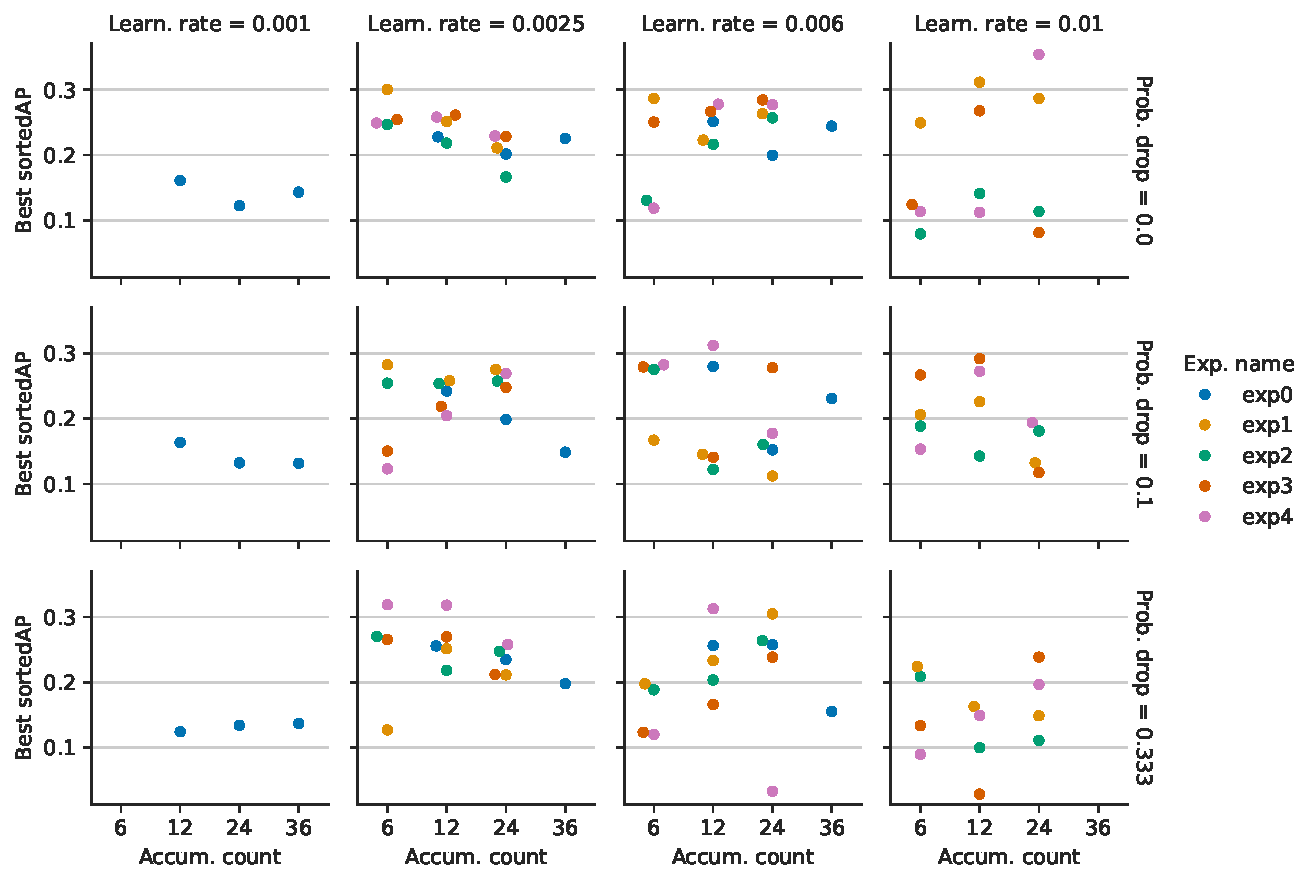
\includegraphics{index_files/figure-pdf/fig-training-parameters-experiments-output-1.pdf}

}

\caption{\label{fig-training-parameters-experiments}Results with
different training parameters for all experiments}

\end{figure}%

\textsubscript{Source:
\href{https://ZokszY.github.io/Geodan-internship-report/index.qmd.html}{Article
Notebook}}

In the next graph (Figure~\ref{fig-training-parameters-data}), we can
see more results for the same experiments. Here, the results are colored
according to the data that we use to evaluate the model. In blue, we see
the value of sortedAP when we evaluate the model with the CHM layers
data and dummy zero arrays as RGB/CIR data. These dummy arrays are also
those that are used as input when one of the channel is dropped during
training, when we have a drop probability larger than 0. Some
interesting patterns appear in some of the cells in this plot. Firstly,
it looks like randomly dropping one of the two inputs with the same
probability has a much larger influence over the results using RGB/CIR
than CHM. While CHM gives better results than RGB/CIR when always
training using everything, RGB/CIR seems to perform better alone when
also trained alone, even outperforming the combination of both inputs in
certain cases.

\textsubscript{Source:
\href{https://ZokszY.github.io/Geodan-internship-report/index.qmd.html}{Article
Notebook}}

\begin{figure}[H]

\centering{

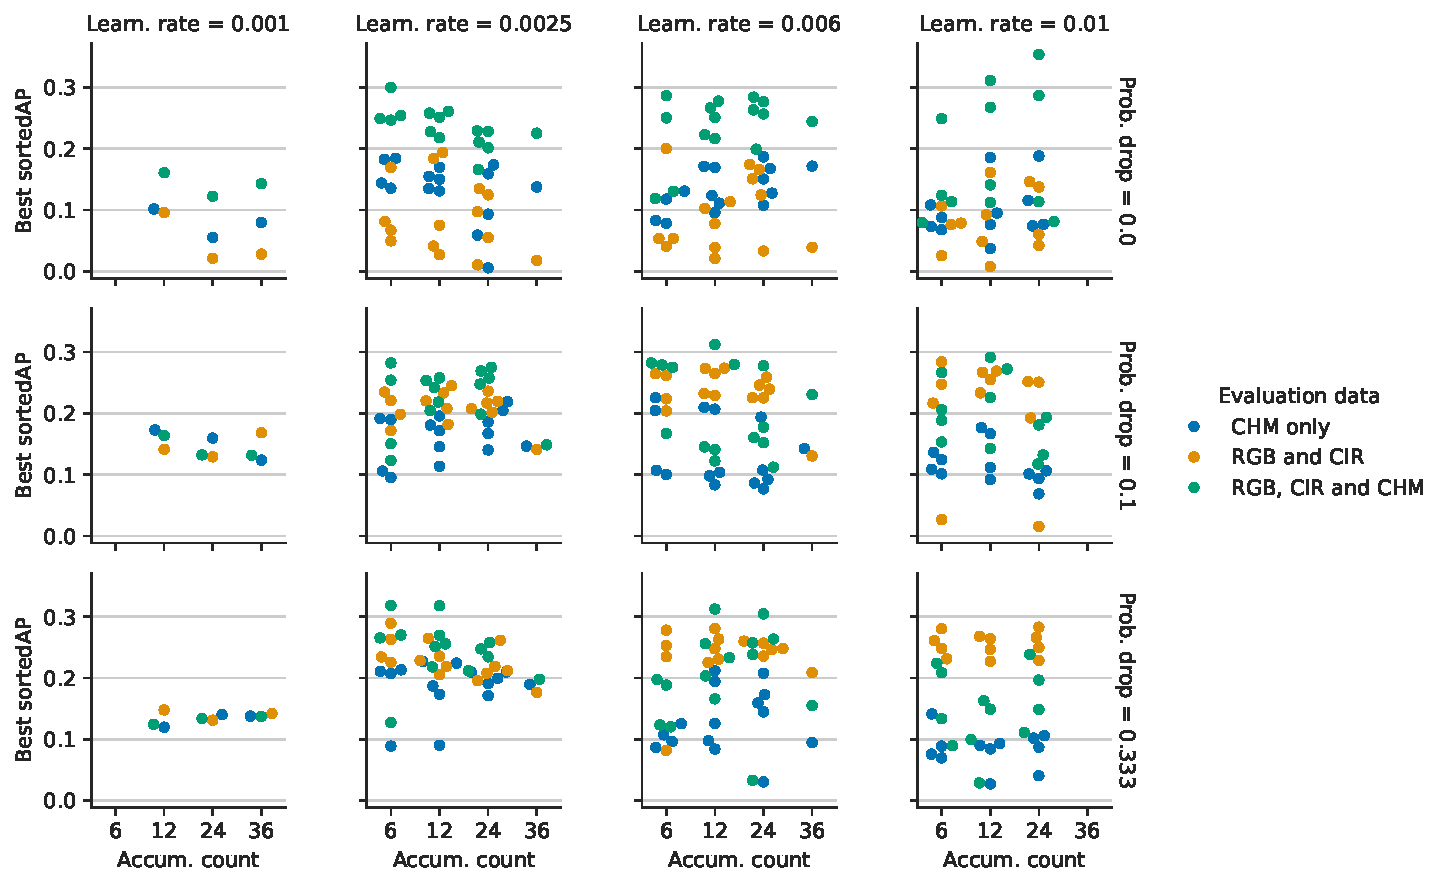
\includegraphics{index_files/figure-pdf/fig-training-parameters-data-output-2.pdf}

}

\caption{\label{fig-training-parameters-data}Results with different
training parameters for all evaluation data setups}

\end{figure}%

\textsubscript{Source:
\href{https://ZokszY.github.io/Geodan-internship-report/index.qmd.html}{Article
Notebook}}

From the results of this experiment, I decided to pick the following
parameters for the next experiments:

\begin{itemize}
\tightlist
\item
  Initial learning rate: 0.004
\item
  Drop probability: 0
\item
  Accumulation count: 10
\end{itemize}

\subsection{Data used}\label{data-used}

\subsection{CHM layers}\label{chm-layers}

\subsection{Hard trees}\label{hard-trees}

\section{Discussion}\label{discussion}

\subsection{Dataset}\label{dataset}

\begin{itemize}
\tightlist
\item
  DeepForest: A Python package for RGB deep learning tree crown
  delineation \autocite{DeepForest}: uses only RGB data to detect trees,
  but uses LiDAR to create millions of annotations of moderate quality
  to pre-train the model, before using around 10,000 hand-annotations to
  finalize and specialize the training on a certain area.
\end{itemize}

\subsection{Combination of data types}\label{combination-of-data-types}

\section*{Conclusion}\label{conclusion}
\addcontentsline{toc}{section}{Conclusion}

Blablabla

\textsubscript{Source:
\href{https://ZokszY.github.io/Geodan-internship-report/index.qmd.html}{Article
Notebook}}


\printbibliography[title=Bibliography]



\end{document}
